\chapter{The Variable Library}

The variable library is a repository for variables defined in the system.  These variables can be used generally throughout the system, whether for defining variables to help predict property values or household location choices, or to compute indicators that are useful for evaluating simulation results, like change in open space or in population density.  Since it provides a resource that is used throughout the GUI, we access it from the tools menu on the menu bar at the top of the main window, as in Figure \ref{fig:variable-library-menu}.  The screenshot in Figure \ref{fig:variable-library-main} shows a popup window that appears once a user selects the variable library option on the tools menu.  Note that the contents of it depend on what project is loaded.  In this case, we have the eugene\_parcel project loaded, and see the variables that are initially available.  

\begin{figure}[htp]
\begin{center}
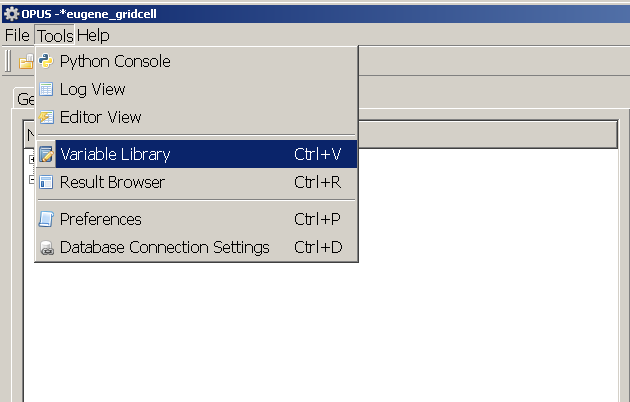
\includegraphics[scale=0.6]{part-gui/images/model-manager-variable-library-menu.png}
\end{center}
\caption{Variable Library Menu}
\label{fig:variable-library-menu}
\end{figure}

\begin{figure}[htp]
\begin{center}
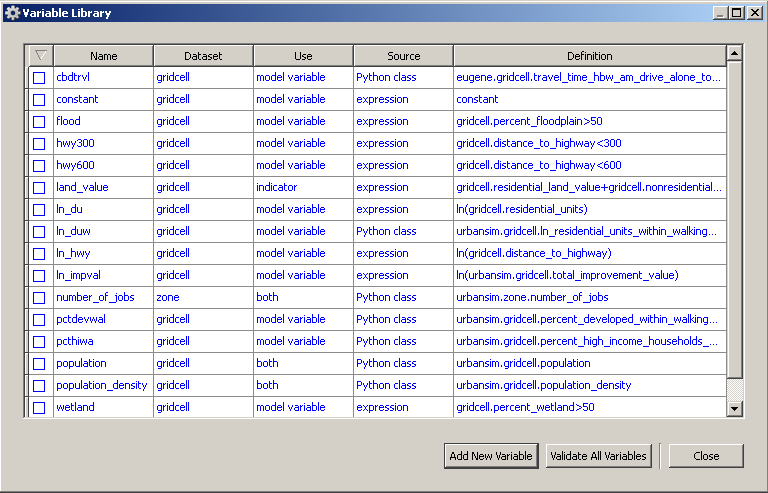
\includegraphics[scale=0.6]{part-gui/images/model-manager-variable-library-main.png}
\end{center}
\caption{Variable Library Main Window}
\label{fig:variable-library-main}
\end{figure}

Note the buttons at the bottom of this window to add new variables or validate all variables.  Adding a new variable is straightforward, using the GUI and the OPUS expression language, which provides a simple syntax for defining variables.  Notice examples of these in the variable library window, in the right-most column.  Expressions are simply functions of one or more primary attributes (think of these as columns in the input database) and possibly functions of other expressions as well.  For example, the expression for wetland is defined as gridcell.percent_wetland>50.  This defines the creation of a true/false, or boolean, variable that is interpreted as 1 if the gridcell has more than 50 percent coverage by wetland, 0 otherwise. Chapter \ref{chap:creating-variables} provides a more thorough introduction to the use of expressions and variables.

If you click on the add new variable button at the bottom of the variable library window, it opens a dialog box as shown in Figure \ref{fig:new-variable}.  The top entry is the name you want to use for the variable.  Let's say we want to create a new variable that is a log of population density.  We already have a population density variable defined by gridcell, so we can just take the log of this value.  Let's name the variable ln\_population\_density, leave the middle selection as \emph{expression}, and fill in a simple expression in the definition area: \emph{ln(gridcell.population_density)}.  Note that the dialog box provides two buttons to help you check your new variable.  The check syntax button tests whether the expression you have entered passes the Python and expression syntax checkers -- in other words, is it syntactically correct.  The second allows you to test whether if you apply this expression to your available data, it can successfully compute a result.  This is very helpful in determining whether you might have referred to a data element that is not present, or is otherwise not computable with your data.  In short, these two tools allow thoroughly testing whether the variables are in a state that can be computed on the available data.

\begin{figure}[htp]
\begin{center}
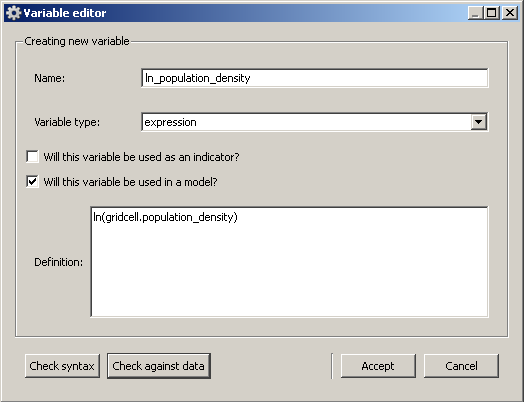
\includegraphics[scale=0.6]{part-gui/images/model-manager-variable-library-new-variable.png}
\end{center}
\caption{Adding a New Variable}
\label{fig:variable-library-new-variable}
\end{figure}